%%%%%%%%%%%%%%%%%%%%%%%%%%%%%%%%%%%%%%%%%%%%%%%%%%%%%%%%%%%%%%%%%%%%%%%%%%%%%%%%%%%%%%%%%%%%%%%%%
% Chapter 2: Background   (the \chapter command is in main.tex)
%%%%%%%%%%%%%%%%%%%%%%%%%%%%%%%%%%%%%%%%%%%%%%%%%%%%%%%%%%%%%%%%%%%%%%%%%%%%%%%%%%%%%%%%%%%%%%%%%

This chapter introduces the battery ideas and the filtering theory used in the rest of the report. Each battery idea in Section~\ref{sec:bg_battery} appears directly in the equations of Chapter~\ref{ch:method}. Section~\ref{sec:bg_kf} explains the Kalman filter and its extended form, and Section~\ref{sec:bg_example} works through one filter step with real numbers. Section~\ref{sec:bg_related} reviews related work.

%--------------------------------------------------------------------------------------------------
\section{Battery basics}\label{sec:bg_battery}
%--------------------------------------------------------------------------------------------------

\subsection{State of charge and capacity}\label{sec:bg_soc}

The \emph{capacity} $C_n$ is the amount of charge a full battery can deliver, measured in ampere-hours (Ah). A 5\,Ah battery can supply 5\,A for one hour, or 20\,A for 15 minutes. Capacity falls as a battery ages; an old battery may hold only 80\% of its rated capacity.

The \emph{state of charge} is the fraction of the capacity that remains:
\begin{equation}
  \mathrm{SoC} = \frac{C_{\text{rem}}}{C_n},
  \label{eq:bg_soc}
\end{equation}
where $C_{\text{rem}}$ is the remaining charge in Ah. SoC is 1 (100\%) when full and 0 when empty. Inside all equations SoC is kept as a fraction; it is converted to a percentage only for plots and tables.

\subsection{Open-circuit voltage curve}\label{sec:bg_ocv}

When a battery has rested with no current flowing, its voltage depends only on its SoC. This resting voltage is the \emph{open-circuit voltage} (OCV), and the function $\mathrm{OCV}(\mathrm{SoC})$ is the OCV curve. Figure~\ref{fig:bg_ocv_tangent} shows the curve used in this project.

\begin{figure}[htbp]
  \centering
  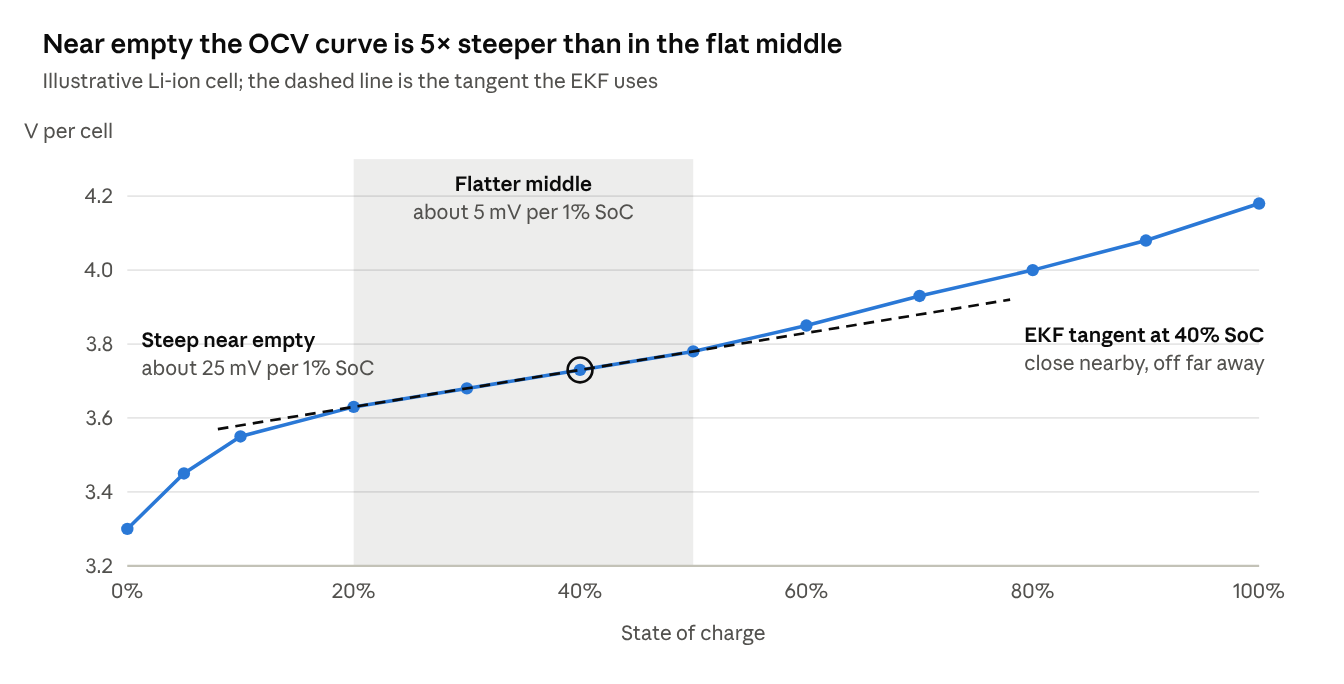
\includegraphics[width=0.85\textwidth]{fig2_ocv_curve.png}
  \caption{OCV curve of one lithium-ion cell (the 12-point table used in this project). The curve is steep near empty and much flatter between about 20\% and 50\% SoC. The dashed tangent at 40\% SoC is close to the curve nearby and drifts away far from it; the EKF only ever uses the tangent near its current estimate.}
  \label{fig:bg_ocv_tangent}
\end{figure}

Two features of the curve matter for estimation.
\begin{itemize}
  \item \textbf{It is curved.} A straight line cannot describe it over the whole SoC range. This is the reason a plain Kalman filter is not enough and an extended one is needed (Section~\ref{sec:bg_ekf}).
  \item \textbf{Its slope changes.} Between 0\% and 10\% SoC the table rises by about 25\,mV per 1\% SoC; between 20\% and 40\% it rises by only 5\,mV per 1\% SoC. Where the curve is flat, a small voltage error corresponds to a large SoC error, so the voltage carries less information about the SoC. A good filter should become less certain there.
\end{itemize}

\subsection{Internal resistance and voltage sag}\label{sec:bg_r0}

A battery behaves as if it contains a small resistor, the \emph{ohmic resistance} $R_0$. When a current $I$ flows (positive for discharge), the terminal voltage drops instantly by
\begin{equation}
  \Delta V_{R_0} = R_0\, I .
  \label{eq:bg_sag}
\end{equation}
With $R_0 = 8$\,m$\Omega$ and $I = 30$\,A (a typical take-off current for the drone in this project), the drop is 0.24\,V per cell. This \emph{voltage sag} fools simple voltage-based fuel gauges: during take-off the battery looks emptier than it really is.

\subsection{Polarisation}\label{sec:bg_rc}

On top of the instant drop, a slower extra drop builds up over tens of seconds of heavy load and fades when the load eases. It is caused by slow chemical processes inside the cell. It is modelled by a resistor $R_1$ in parallel with a capacitor $C_1$. The voltage across this pair is the \emph{polarisation voltage} $V_1$, and it obeys
\begin{equation}
  C_1 \frac{dV_1}{dt} = I - \frac{V_1}{R_1}.
  \label{eq:bg_rc}
\end{equation}
Under a constant current, $V_1$ moves exponentially towards $R_1 I$ with time constant $\tau_1 = R_1 C_1$. For $R_1 = 6$\,m$\Omega$ and $C_1 = 5000$\,F, $\tau_1 = 30$\,s. Nobody measures $V_1$, so the filter must estimate it.

\subsection{The equivalent circuit}\label{sec:bg_ecm}

Putting these pieces together gives the equivalent circuit of Figure~\ref{fig:bg_circuit}: an OCV source in series with $R_0$ and the $R_1$--$C_1$ pair. The voltage at the battery terminals, which is what the voltage sensor reads, is
\begin{equation}
  V = \mathrm{OCV}(\mathrm{SoC}) - R_0\, I - V_1 .
  \label{eq:bg_terminal}
\end{equation}
Only $V$ and $I$ are measured. The filter has to infer SoC and $V_1$ from them.

\begin{figure}[htbp]
  \centering
  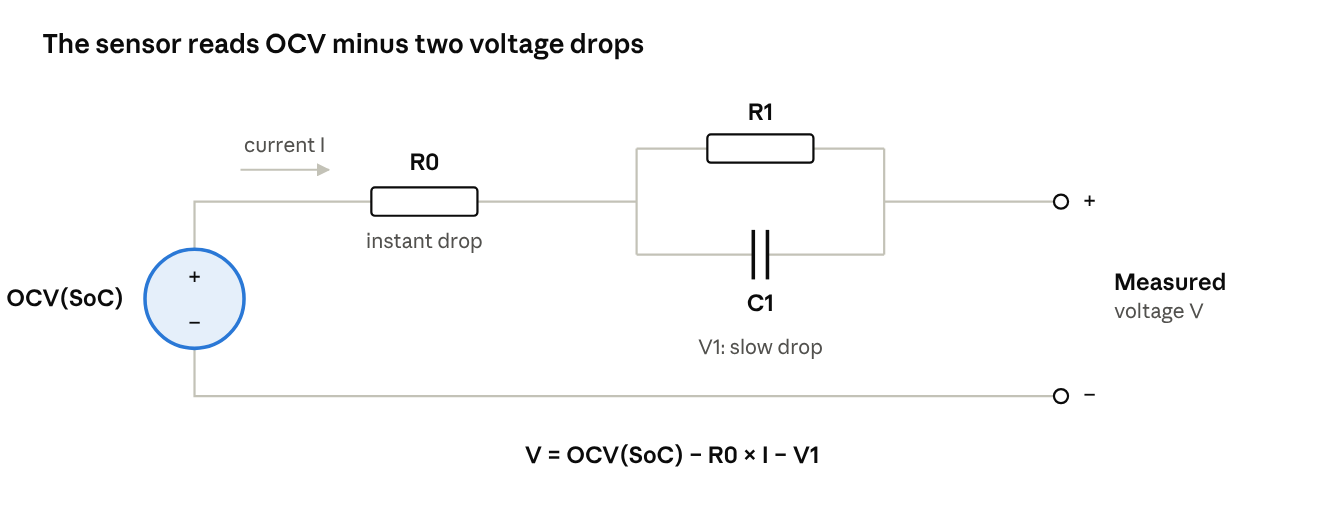
\includegraphics[width=0.85\textwidth]{fig3_equivalent_circuit.png}
  \caption{One-RC equivalent circuit of a cell. The sensor reads the OCV minus two drops: an instant drop across $R_0$ and a slow drop $V_1$ across the $R_1$--$C_1$ pair. This is the model the EKF uses; the simulated ``true'' battery adds a second, slower RC pair (Section~\ref{sec:m_truth_vs_filter}).}
  \label{fig:bg_circuit}
\end{figure}

\subsection{Charge counting and why it drifts}\label{sec:bg_cc}

The obvious way to track SoC is to start from a known value and subtract the charge drawn. This is \emph{charge counting}, also called Coulomb counting. With a time step $\Delta t$ in seconds, a current $I_k$ in amperes drawn during step $k$, and $\mathrm{SoC}_k$ the SoC at the end of step $k$,
\begin{equation}
  \mathrm{SoC}_{k} = \mathrm{SoC}_{k-1} - \frac{I_k\, \Delta t}{3600\, C_n}.
  \label{eq:bg_cc}
\end{equation}
The factor 3600 converts seconds to hours, because $C_n$ is in Ah. The method is simple, but it has three weaknesses.
\begin{itemize}
  \item \textbf{Wrong start.} If the initial SoC is wrong, the error stays for the whole flight; nothing in \eqref{eq:bg_cc} corrects it.
  \item \textbf{Sensor bias.} If the current sensor reads a constant $b$ amperes too high, the SoC error grows linearly with time:
  \begin{equation}
    e(t) = -\frac{b\, t}{3600\, C_n}.
    \label{eq:bg_cc_drift}
  \end{equation}
  A 0.5\,A bias over 15 minutes is 0.125\,Ah, which is 2.5\% of a 5\,Ah battery.
  \item \textbf{Wrong capacity.} An aged battery has a smaller $C_n$ than the counter assumes, so it empties faster than the counter predicts.
\end{itemize}
The EKF corrects all three by using the voltage as a second, independent clue. Charge counting is kept as a baseline for comparison.

%--------------------------------------------------------------------------------------------------
\section{From the Kalman filter to the Extended Kalman Filter}\label{sec:bg_kf}
%--------------------------------------------------------------------------------------------------

\subsection{The idea}\label{sec:bg_kf_idea}

Imagine walking through a dark room while counting steps. Each step adds a little error, so your sense of position slowly drifts. Now and then you touch a wall whose position you know, and you correct yourself. If your step counting is sloppy, you trust the wall more; if the wall touch is vague, you trust your counting more. A Kalman filter formalises this balance. For the drone, counting charge (Equation~\ref{eq:bg_cc}) plays the role of counting steps, and reading the voltage (Equation~\ref{eq:bg_terminal}) plays the role of touching the wall.

\subsection{The state-space model}\label{sec:bg_ss}

The filter works with a \emph{state vector} $x_k$ that holds the hidden quantities at time step $k$ (for example SoC and $V_1$). A known \emph{input} $u_k$ (here the measured current) drives the state forward, and a \emph{measurement} $z_k$ (here the measured voltage) depends on the state:
\begin{align}
  x_k &= f(x_{k-1}, u_k) + w_k, & w_k &\sim \mathcal{N}(0, Q), \label{eq:bg_process}\\
  z_k &= h(x_k, u_k) + v_k,     & v_k &\sim \mathcal{N}(0, R). \label{eq:bg_measurement}
\end{align}
Here $f$ is the \emph{process model} (how the state changes in one step) and $h$ is the \emph{measurement model} (what the sensor should read, given the state). The terms $w_k$ and $v_k$ are random errors with zero mean. $\mathcal{N}(0, Q)$ denotes a Gaussian (bell-shaped) distribution with zero mean and covariance $Q$. $Q$ is the \emph{process-noise covariance} and $R$ is the \emph{measurement-noise covariance}. In this report $Q$ and $R$ always mean these two matrices; the battery capacity is written $C_n$ and the resistors are $R_0$, $R_1$.

\subsection{The Kalman filter loop}\label{sec:bg_kf_loop}

The filter keeps two things: an estimate $\hat{x}_k$ of the state, and a covariance matrix $P_k$ that describes how uncertain that estimate is. The diagonal of $P_k$ holds the variance of each state; the off-diagonal entries say how the errors of different states are linked. For example, ``SoC $= 62\% \pm 2\%$'' means $\hat{x} = 0.62$ and $\sqrt{P} = 0.02$ for a one-state filter.

When $f$ and $h$ are linear, $f(x, u) = F x + B u$ and $h(x) = H x$ for constant matrices $F$, $B$ and $H$. Each time step then has two parts (Figure~\ref{fig:bg_ekf_loop}).

\textbf{Predict.} Push the estimate forward with the model. The uncertainty grows, because the model and the input are imperfect:
\begin{align}
  \hat{x}_k^- &= F \hat{x}_{k-1} + B u_k, \label{eq:bg_kf_xpred}\\
  P_k^- &= F P_{k-1} F^{\top} + Q. \label{eq:bg_kf_ppred}
\end{align}
The superscript ``$-$'' means ``before the measurement is used''.

\textbf{Update.} Compare the measurement with what the model expected. The difference is the \emph{innovation} $\tilde{y}_k$, the filter's ``surprise''. Move the estimate to explain part of the surprise; the uncertainty shrinks:
\begin{align}
  \tilde{y}_k &= z_k - H \hat{x}_k^-, \label{eq:bg_kf_innov}\\
  S_k &= H P_k^- H^{\top} + R, \label{eq:bg_kf_s}\\
  K_k &= P_k^- H^{\top} S_k^{-1}, \label{eq:bg_kf_gain}\\
  \hat{x}_k &= \hat{x}_k^- + K_k \tilde{y}_k, \label{eq:bg_kf_xupd}\\
  P_k &= (\mathbb{I} - K_k H) P_k^-. \label{eq:bg_kf_pupd}
\end{align}
$S_k$ is the expected size (variance) of the innovation, $K_k$ is the \emph{Kalman gain}, and $\mathbb{I}$ is the identity matrix. When the model is linear and the noise Gaussian, this filter gives the best possible estimate in the least-squares sense~\cite{simon2006optimal,welch2006intro}.

\begin{figure}[htbp]
  \centering
  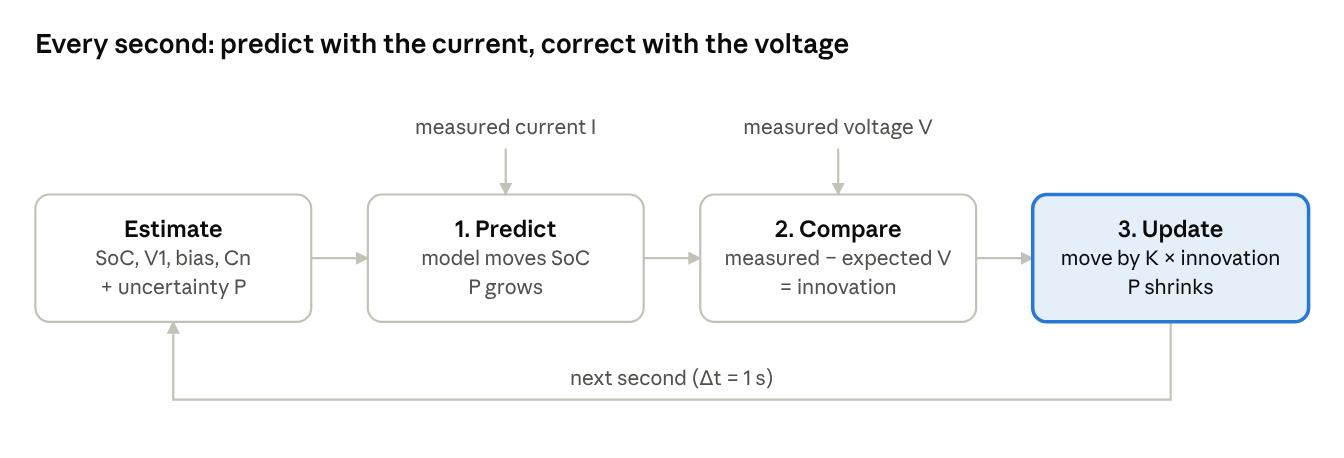
\includegraphics[width=0.85\textwidth]{fig4_ekf_loop.png}
  \caption{The filter loop, repeated every second. The measured current drives the prediction (uncertainty $P$ grows); the measured voltage drives the correction (uncertainty $P$ shrinks).}
  \label{fig:bg_ekf_loop}
\end{figure}

\subsection{The Kalman gain: a trust balance}\label{sec:bg_gain}

The gain $K_k$ in \eqref{eq:bg_kf_gain} decides how far the estimate moves towards what the measurement suggests. Its behaviour follows from the equation and is summarised in Table~\ref{tab:bg_gain}.

\begin{table}[htbp]
  \centering
  \caption{How the Kalman gain reacts to different situations.}
  \label{tab:bg_gain}
  \begin{tabular}{@{}p{0.46\textwidth}lp{0.34\textwidth}@{}}
    \toprule
    Situation & $K$ & What the filter does \\
    \midrule
    Prediction very uncertain ($P^-$ large) & Large & Follows the measurement \\
    Sensor very noisy ($R$ large) & Small & Keeps its prediction \\
    Measurement says little about the state ($H$ small, e.g.\ flat OCV) & Small & Barely changes the state \\
    \bottomrule
  \end{tabular}
\end{table}

\subsection{The tuning knobs Q and R}\label{sec:bg_qr}

$Q$ says how much the filter distrusts its model at each step, and $R$ says how much it distrusts the sensor. A large $Q$ makes the filter react quickly but jumpily; a large $R$ makes it smooth but slow. $R$ can usually be set from the sensor's datasheet noise. $Q$ is harder; Section~\ref{sec:m_ekf_q} derives most of it from the current-sensor noise instead of guessing it.

\subsection{What ``Extended'' adds}\label{sec:bg_ekf}

The equations above need linear $f$ and $h$: only then does a Gaussian uncertainty stay Gaussian. The battery's measurement model \eqref{eq:bg_terminal} contains $\mathrm{OCV}(\mathrm{SoC})$, which is curved. The EKF deals with this by linearising: at every step it replaces $f$ and $h$ by their tangent (first-order Taylor) approximation at the current estimate. The slopes go into the \emph{Jacobian} matrices
\begin{equation}
  F_k = \left.\frac{\partial f}{\partial x}\right|_{\hat{x}_{k-1},\,u_k},
  \qquad
  H_k = \left.\frac{\partial h}{\partial x}\right|_{\hat{x}_k^-,\,u_k}.
  \label{eq:bg_jacobians}
\end{equation}
The EKF then runs the same loop as the KF, with two changes: the state and the expected measurement are computed with the full nonlinear functions, $\hat{x}_k^- = f(\hat{x}_{k-1}, u_k)$ and $\tilde{y}_k = z_k - h(\hat{x}_k^-, u_k)$; and the Jacobians $F_k$ and $H_k$ replace $F$ and $H$ in the covariance and gain equations \eqref{eq:bg_kf_ppred} and \eqref{eq:bg_kf_s}--\eqref{eq:bg_kf_pupd}.

For the battery, the key entry of $H_k$ is the slope $d\,\mathrm{OCV}/d\,\mathrm{SoC}$ at the current SoC estimate. The tangent line in Figure~\ref{fig:bg_ocv_tangent} is exactly what the EKF uses.

Linearisation works well when the function is smooth and the uncertainty is small compared with the scale over which the slope changes. It works badly with sharp bends or very large uncertainty. In those cases the unscented Kalman filter (UKF) or a particle filter (PF), which do not rely on a single tangent, usually do better, at a higher computational cost~\cite{simon2006optimal}.

%--------------------------------------------------------------------------------------------------
\section{A worked example: one EKF step by hand}\label{sec:bg_example}
%--------------------------------------------------------------------------------------------------

To make the loop concrete, this section works through one predict--update step with real numbers, using a deliberately simple model (the script \texttt{learning/day1\_ekf\_by\_hand.m}).

\subsection{Set-up}

The state is the SoC only ($x = \mathrm{SoC}$). There is no polarisation, no bias state, and the capacity is known: $C_n = 5$\,Ah, $R_0 = 8$\,m$\Omega$. The time step is $\Delta t = 10$\,s, chosen so that the SoC change is easy to see. The process noise is $Q = 10^{-6}$ and the measurement noise is $R = (0.01\text{\,V})^2 = 10^{-4}$\,V$^2$ (a 10\,mV sensor). Near 79\% SoC the OCV curve is approximated by a straight line through (70\%, 3.93\,V) with slope 0.7\,V per unit SoC (7\,mV per 1\% SoC). The measurement model is $V = \mathrm{OCV}(\mathrm{SoC}) - R_0 I$.

The filter starts at $\mathrm{SoC} = 80\% \pm 5\%$, so $\hat{x} = 0.80$ and $P = 0.05^2$. During the step the measured current is 20\,A, and at the end the measured voltage is 3.80\,V.

\subsection{The step}

\textbf{Predict.} Charge counting \eqref{eq:bg_cc} gives
\[
  \hat{x}^- = 0.80 - \frac{20 \times 10}{3600 \times 5} = 0.7889 \;(78.89\%).
\]
Here $F = 1$, so $P^- = P + Q = 0.05^2 + 10^{-6}$.

\textbf{Compare.} The voltage the model expects at the predicted SoC is $3.93 + 0.7\,(0.7889 - 0.70) - 0.008 \times 20 = 3.8322$\,V. The measured voltage is 3.80\,V, so the innovation is $\tilde{y} = 3.80 - 3.8322 = -0.0322$\,V. The battery reads 32\,mV lower than expected.

\textbf{Update.} The measurement Jacobian is the OCV slope, $H = 0.7$\,V per unit SoC. Then
\[
  S = H^2 P^- + R = 0.001325\text{\,V}^2, \qquad
  K = \frac{P^- H}{S} = 1.321\text{\,V}^{-1},
\]
and the updated estimate is $78.89\% + 1.321 \times (-0.0322) \times 100\% = 74.63\%$, with standard deviation $\sqrt{(1 - KH)P^-} = 1.37\%$.

\subsection{What the numbers mean}

$K$ is not a pure number here: it converts volts of surprise into SoC, so its unit is ``SoC per volt''. A gain above 1 is therefore not a problem. The useful dimensionless quantity is $KH = 0.925$. The 32\,mV surprise, divided by the slope of 7\,mV per 1\% SoC, suggests that the SoC is about 4.6 percentage points lower than predicted. The filter moves 92.5\% of the way towards that suggestion. It trusts the voltage so much because its prior was vague ($\pm 5\%$) while the sensor is precise (10\,mV corresponds to only about 1.4\% SoC at this slope). In one step the uncertainty falls from 5\% to 1.37\%.

Table~\ref{tab:bg_knobs} repeats the same step with the knobs turned. A noisier sensor or a more confident prior both reduce the gain, exactly as Table~\ref{tab:bg_gain} predicts.

\begin{table}[htbp]
  \centering
  \caption{Kalman gain for the same step under three settings (learning script, Part 2).}
  \label{tab:bg_knobs}
  \begin{tabular}{@{}lc@{}}
    \toprule
    Setting & $K$ (V$^{-1}$) \\
    \midrule
    Baseline: 10\,mV sensor, prior $\pm 5\%$ & 1.321 \\
    Noisy sensor: 50\,mV, prior $\pm 5\%$ & 0.470 \\
    Confident prior: 10\,mV sensor, prior $\pm 1\%$ & 0.473 \\
    \bottomrule
  \end{tabular}
\end{table}

\subsection{A ten-minute discharge}

Part 3 of the same script runs the one-state filter for 10 minutes ($\Delta t = 1$\,s) at a constant 15\,A. The true battery starts at 75\%, but both the EKF and charge counting wrongly start at 80\%. The current sensor has a bias of 0.3\,A and noise of 0.2\,A; the voltage sensor has 10\,mV noise. The full 12-point OCV table is used (with linear interpolation). The process noise is set from the current noise, $Q = \left(\Delta t/(3600 C_n)\right)^2 \sigma_I^2 + 10^{-9}$, where $\sigma_I$ is the current-noise standard deviation; this is a one-state preview of the derivation in Section~\ref{sec:m_ekf_q}.

At the end of the 10 minutes the SoC error was $-0.12\%$ for the EKF and $+4.01\%$ for charge counting. The counting error is what the theory predicts: the $+5\%$ start error never goes away, and the 0.3\,A bias over 600\,s removes 0.05\,Ah, which is 1\% of 5\,Ah, from the estimate. The EKF does not model the bias in this simple version, yet its error stays small, because the voltage pulls the estimate back towards the truth at every step.

This is a best case. Apart from the bias, the simulated battery in this exercise is exactly the filter's own model. The full project tests the filter against a battery that differs from its model (Section~\ref{sec:m_truth_vs_filter}).

%--------------------------------------------------------------------------------------------------
\section{Related work}\label{sec:bg_related}
%--------------------------------------------------------------------------------------------------

\textbf{EKF for battery management.} Plett's three-part paper~\cite{plett2004part1,plett2004part2,plett2004part3} is the classic reference for EKF-based battery state estimation. Part~1 gives the background, Part~2 covers cell modelling and identification, and Part~3 covers state and parameter estimation, applied to lithium-ion polymer battery packs for hybrid electric vehicles. The idea of adding unknown parameters, such as resistance or capacity, to the state vector and estimating them alongside the SoC, used in this project, follows this line of work. Plett's textbook~\cite{plett2015bms} treats equivalent-circuit models and their estimation in depth. MathWorks provides an EKF battery-estimation example in MATLAB~\cite{mathworks_ekf_battery}, which is useful as a cross-check for the code in this project.

\textbf{Estimation theory.} Simon~\cite{simon2006optimal} covers the Kalman filter, the EKF, the UKF and the particle filter, including their assumptions and failure modes. Welch and Bishop~\cite{welch2006intro} give a short introduction to the Kalman filter and the EKF.

\textbf{Battery estimation for drones.} Several works apply these ideas to unmanned aerial vehicles (UAVs). An EKF has been used for SoC estimation in UAV applications~\cite{hal_uav_ekf}. Prognostic algorithms that predict the remaining flying time of electric unmanned vehicles have been verified~\cite{ijphm_flight_time}; remaining flying time is the quantity an RTH decision ultimately depends on. Dibbern et al.~\cite{purdue_jate_comparison} compared an EKF, a UKF and Coulomb counting for a multirotor UAV battery on a delivery mission and a facade-inspection mission. They found the UKF more accurate than the EKF, and found that identifying the battery parameters mattered more for SoC accuracy than the dynamic load.

\textbf{Public data.} Real flight and duty-cycle data are available for future validation: in-flight voltage and current logs from 209 package-delivery flights of a DJI Matrice 100 quadcopter~\cite{cmu_dji_dataset}, an eVTOL battery dataset with take-off, cruise and landing duty cycles~\cite{cmu_evtol_dataset,cmu_evtol_paper}, and LG 18650HG2 cell data intended for testing Kalman-filter SoC algorithms~\cite{mcmaster_lg_hg2}. This project uses simulation only (Section~\ref{sec:m_truth_vs_filter}), so that the true SoC is known and every error can be measured exactly.

\textbf{Focus of this project.} The project combines an EKF that learns the cell resistance alongside the SoC (with an observability study of also learning the sensor bias and capacity) with an RTH rule that uses the filter's uncertainty, not only its estimate. Both are tested against a deliberately mismatched battery model and simpler baselines.
